%% draft.tex
%% "Measuring Causal Effects under Opaque Targeting:
%%  Point and Partial Identification in Overlay Experiments"
%%
%% Target: Management Science / Marketing Science
%% Format modeled on Ye et al. (2025, Management Science)

\documentclass[12pt]{article}
\usepackage[utf8]{inputenc}
\usepackage{amsmath, amssymb, amsthm, mathtools, bm}
\usepackage[margin=1in]{geometry}
\usepackage{setspace}
\usepackage{booktabs}
\usepackage[authoryear,round]{natbib}
\usepackage{hyperref}
\usepackage{graphicx}
\usepackage{caption}
\usepackage{subcaption}
\usepackage{array}
\usepackage{xcolor}
\doublespacing

%% Theorem environments
\newtheorem{assumption}{Assumption}
\newtheorem{proposition}{Proposition}
\newtheorem{theorem}{Theorem}
\newtheorem{lemma}{Lemma}
\newtheorem{corollary}{Corollary}
\newtheorem{remark}{Remark}
\newtheorem{definition}{Definition}

%% Notation shortcuts
\newcommand{\E}{\mathbb{E}}
\newcommand{\Prob}{\mathbb{P}}
\newcommand{\indep}{\perp\!\!\!\perp}
\newcommand{\ATT}{\mathrm{ATT}}
\newcommand{\ATE}{\mathrm{ATE}}
\newcommand{\ITT}{\mathrm{ITT}}
\newcommand{\ATU}{\mathrm{ATU}}
\newcommand{\MTE}{\mathrm{MTE}}

% ─────────────────────────────────────────────────────────────────────────────
\title{Measuring Causal Effects under Opaque Targeting:\\
       Point and Partial Identification in Overlay Experiments}
\author{Qifan Han\thanks{Author affiliation and contact information.}}
\date{\today}
% ─────────────────────────────────────────────────────────────────────────────

\begin{document}
\maketitle

% ─────────────────────────────────────────────────────────────────────────────
\begin{abstract}
Large digital platforms run hundreds of simultaneous advertising experiments
every day, using proprietary algorithms to decide which users receive each
campaign. From the perspective of an advertiser or external researcher, the
platform's targeting logic is a black box. We study a practical experimental
design---the \emph{overlay experiment}---in which the experimenter randomizes
campaign eligibility while the platform continues to apply its own targeting
rule. We show that the overlay experiment identifies the Average Treatment
Effect on the Treated (ATT), the causal effect for the users the platform
actually selects, and not the population Average Treatment Effect (ATE). The
ATT can substantially exceed the ATE when the platform's algorithm selects
users with the highest expected response---a form of algorithmic
cherry-picking. We quantify this gap through the \emph{Selection Ratio},
$R = \mathrm{ATT}/\mathrm{ATE}$, which is identified up to sharp bounds
$R \in [1,\, 1/p]$ where $p$ is the observed targeting rate. When an
additional variable that shifts targeting intensity without affecting outcomes
directly is available---for instance, different advertising budget levels
across geographic markets---we show how to point-identify the full
heterogeneous treatment effect schedule and the population ATE. Monte Carlo
experiments using three concrete platform targeting scenarios confirm that
the overlay estimator correctly recovers ATT while standard alternatives
(ordinary least squares, plain intent-to-treat) fail persistently.
\end{abstract}

\clearpage
% ─────────────────────────────────────────────────────────────────────────────
\section{Introduction}
\label{sec:intro}
% ─────────────────────────────────────────────────────────────────────────────

How effective is an advertising campaign? This question---central to marketing
science---has grown harder to answer as advertising increasingly occurs on
large digital platforms that simultaneously manage thousands of campaigns,
each targeting users through proprietary recommendation algorithms. The gold
standard for causal inference is a randomized experiment, but running a
clean experiment on a platform with opaque targeting creates a subtle
identification problem that practitioners have not fully appreciated.

Consider the following concrete scenario, which we formalize in this paper.
A direct-to-consumer brand purchases advertising inventory on Meta and wants
to measure the effect of its campaign on purchases. Meta's algorithm
decides, using its own optimization logic, which of the brand's
``targeted'' users to actually show the ad. The brand can randomize
\emph{campaign eligibility}---for instance, by randomly activating or
pausing the campaign for different user segments---but within the eligible
set, Meta's algorithm continues to select whom it shows the ad to. This
is the structure of an \emph{overlay experiment}: the experimenter's
randomization is overlaid on top of the platform's opaque targeting rule.

The same structure appears in two other practically important settings.
First, within a firm, different teams often run experiments on the same
users simultaneously. A marketing team's coupon overlay is applied on top
of the recommendation team's personalization algorithm, without either
team seeing the other's targeting logic. Second, in platform auditing and
regulation, external researchers or regulators who cannot control the
platform's algorithm can only randomize incentives or access for a sample
of users---observing outcomes while the platform's own system continues to
operate. In all three settings, the experimenter's realized treatment
equals
\begin{equation}
  W_i = D_i \cdot Z_i,
  \label{eq:overlay}
\end{equation}
where $D_i \in \{0,1\}$ is the platform's latent targeting decision and
$Z_i \in \{0,1\}$ is the experimenter's randomization. Treatment occurs
only when both the platform intends to treat ($D_i=1$) and the
experimenter has made the user eligible ($Z_i=1$). Critically, the
platform's targeting rule governing $D_i$ is unobserved by the experimenter.

\subsection*{The Identification Problem and Main Results}

The overlay structure creates a fundamental identification challenge: because
the platform selects $D_i$ using its own optimization---presumably targeting
users with higher expected responses---the group of users who receive
treatment is not a random sample of the population. Standard intent-to-treat
analysis gives the average effect per eligible user ($\ITT$), which is
smaller than the actual effect on treated users. Naive regression of outcomes
on treatment receipt conflates the treatment effect with the platform's
selection advantage.

We establish three results.

\textbf{Result 1 (Proposition~\ref{prop:att}): The passive overlay identifies
ATT.} Under minimal assumptions---the experimenter's randomization is
independent of the platform's targeting---the ratio $\ITT(x)/p(x)$
identifies the Average Treatment Effect on the Treated, $\ATT(x)$, where
$p(x)$ is the observed targeting rate. The $\ITT$ and $p(x)$ are both
estimable from the experiment; only their ratio correctly accounts for the
platform's selection. This result holds regardless of how the platform's
targeting rule is specified.

\textbf{Result 2 (Theorem~\ref{thm:pointid}): An excluded shifter identifies
the full treatment effect schedule.} When a variable shifts targeting
intensity without directly affecting outcomes---for example, different
advertising budget levels assigned across geographic markets---we show that
the overlay design admits a local instrumental variable representation. The
Marginal Treatment Effect schedule, $\MTE(x,u)$, is identified as the
derivative of the conditional outcome function in the treated arm with
respect to the targeting propensity. Under full support of the propensity,
the population ATE is also identified. This result operationalizes the
Heckman--Vytlacil (2005) local-IV framework in the platform context.

\textbf{Result 3 (Theorem~\ref{thm:sharp}): Without a shifter, sharp bounds
$\ATE(x) \in [\ITT(x), \ATT(x)]$ apply.} When no excluded shifter is
available, we derive the tightest possible bounds on $\ATE$ using two
economically motivated restrictions: (i) the platform prioritizes users
with larger treatment effects (monotone selection on gains), and (ii)
treatment effects are nonnegative. The bounds are \emph{sharp}: both
endpoints are achieved by specific data-generating processes consistent with
the observable data. We introduce the \emph{Selection Ratio}
$R(x) = \ATT(x)/\ATE(x)$ as a practical summary of the platform's
algorithmic efficiency; it is bounded between 1 and $1/p(x)$.

\subsection*{Relation to Ye et al. (2025)}

A growing empirical literature shows that measuring advertising effects
is fundamentally difficult. \citet{lewis2015unfavorable} show that most
advertising experiments are so severely underpowered that even large campaigns
yield near-uninformative estimates of the ATE; targeted experiments that
concentrate power on high-responders partially address this, but they shift
what is estimated from ATE to ATT---a distinction our paper formalizes.
\citet{gordon2019comparison} find that targeting-aware estimators
substantially outperform naive alternatives in large Facebook experiments,
and \citet{gordon2023close} document that observational methods can produce
errors exceeding 100\% of the true effect.

A recent paper by \citet{ye2025deep} addresses a related but distinct
problem: a platform that runs $m$ simultaneous internal A/B tests with an
orthogonal, \emph{known} assignment mechanism wants to estimate the causal
effect of all $2^m$ treatment combinations when only $O(m)$ combinations
are observed. Their Debiased Deep Learning (DeDL) framework solves this
combinatorial identification problem using double machine learning with
structured neural networks.

Our paper is complementary. Ye et al.\ work from the \emph{inside}---the
platform controls and knows all assignment probabilities. We work from the
\emph{outside}---an external advertiser or researcher faces an unknown
platform assignment probability. Our Monte Carlo simulation in
Section~\ref{sec:simulation} directly uses Ye et al.'s generalized sigmoid
outcome model to generate data, but evaluates our overlay estimator in the
setting where the external experimenter has no knowledge of the platform's
internal experiment infrastructure. The two papers together cover the
causal inference landscape for platform experiments from both perspectives.

\subsection*{Practical Takeaways}

Our results carry several immediate implications for practitioners:
\begin{enumerate}
  \item \textbf{Overlay experiments identify ATT, not ATE.} A campaign
    that tests ``well'' on a platform---high in-test lift---may perform
    much more modestly at scale, because the platform's algorithm is
    selecting the users most likely to respond. The gap between ATT and ATE
    measures the platform's cherry-picking advantage.
  \item \textbf{The Selection Ratio bounds the scale-up risk.} With the
    observable targeting rate $p$ and a measured $\ATT$, the ATE is bounded
    in $[p \cdot \ATT, \ATT]$. An advertiser can use this to stress-test
    the business case for scaling a campaign.
  \item \textbf{Budget variation can sharpen the estimate.} Randomizing
    campaign budget across markets---a common practice in multi-market
    testing---provides the excluded shifter needed to point-identify MTE
    and ATE, without requiring any special access to the platform's data.
\end{enumerate}

The remainder of the paper is organized as follows. Section~\ref{sec:lit}
reviews the related literature. Section~\ref{sec:setup} introduces the
model. Section~\ref{sec:passive} presents the ATT identification result.
Section~\ref{sec:pointid} develops point identification with an excluded
shifter. Section~\ref{sec:partial} derives sharp bounds and the Selection
Ratio. Section~\ref{sec:simulation} presents Monte Carlo evidence.
Section~\ref{sec:conclusion} concludes. Formal proofs are in the Appendix.

% ─────────────────────────────────────────────────────────────────────────────
\section{Related Literature}
\label{sec:lit}
% ─────────────────────────────────────────────────────────────────────────────

\subsection*{Local Average and Marginal Treatment Effects}

Our point identification result connects to the literature on heterogeneous
treatment effects under selection. \citet{angrist1994identification} establish
that a binary instrument identifies the Local Average Treatment Effect (LATE),
the effect for compliers. \citet{heckman2005structural} generalize this to
the Marginal Treatment Effect (MTE) framework, which traces the entire
distribution of treatment effects across individuals ordered by their
propensity to be treated. The key identification insight---that the MTE equals
the derivative of the conditional mean outcome with respect to the propensity
score---is at the core of our Theorem~\ref{thm:pointid}. Our contribution is
to show that the overlay design provides a natural and operationally transparent
implementation of this framework: the treated arm directly reveals the platform
propensity score, simplifying estimation relative to the standard local-IV setup.
\citet{vytlacil2002independence} shows that the latent-index structure we adopt
(Assumption~\ref{ass:excluded}) is equivalent to the LATE assumptions, so our
framework invokes no additional restrictions. \citet{carneiro2011estimating}
illustrate the empirical importance of heterogeneity in marginal returns.

\subsection*{Partial Identification}

\citet{manski1990nonparametric} establishes the classic nonparametric bounds
on treatment effects under no assumptions beyond outcome support. Our bounds
in Section~\ref{sec:partial} are tighter because the overlay already identifies
both $\ITT(x)$ and $\ATT(x)$; the question is only how far $\ATE(x)$ can
deviate from $\ATT(x)$. We additionally exploit shape restrictions---monotone
selection on gains and nonnegativity of effects---following
\citet{manski2000monotone}. The result is a sharp interval $[\ITT(x), \ATT(x)]$
that has a transparent economic interpretation.

\subsection*{Simultaneous and Overlapping Platform Experiments}

The engineering infrastructure for running thousands of simultaneous experiments
on large platforms is documented by \citet{tang2010overlapping} for Google and
\citet{kohavi2020trustworthy} for the industry broadly. Their solution---orthogonal
traffic assignment, where each experiment is randomized independently---is the
design that our Assumption~\ref{ass:overlay} requires for the overlay variable
$Z_i$. These papers address the design problem; ours addresses the identification
problem that arises when an external experimenter cannot enforce such a design
and faces an opaque targeting environment.

\subsection*{Combinatorial Experiments}

\citet{ye2025deep} study the problem of estimating the causal effect of all
$2^m$ combinations from $m$ simultaneous platform experiments when only $O(m)$
combinations are observed. Their DeDL framework uses double machine learning
\citep{chernozhukov2018double} with structured deep neural networks. The key
assumption is that the joint assignment mechanism $v(\mathbf{t}|x)$ is
\emph{known} to the platform. Our paper addresses the complementary case where
the external experimenter does not know $v(\mathbf{t}|x)$---or equivalently
$p(x) = \Prob(D_i=1|X_i=x)$---and must rely on their own randomization to
identify causal effects. The two frameworks are complementary: Ye et al.\
identify all cross-experiment interaction effects from the inside, while we
identify the marginal effect for any single experimenter from the outside.

\subsection*{Advertising Measurement and Platform Experiments}

Measuring the causal effect of advertising is a long-standing challenge
in marketing. \citet{lewis2015unfavorable} show that most advertising
experiments are so severely underpowered---relative to the variance of
purchase outcomes---that even very large campaigns yield near-uninformative
confidence intervals for the ATE. This motivates the use of targeted
experiments that concentrate statistical power on high-probability responders,
which is precisely what overlay experiments with platform targeting do:
by concentrating treatment on high-intent users, the platform implicitly
increases the signal-to-noise ratio of the experiment at the cost of
measuring a population-specific effect (ATT rather than ATE). Our paper
formalizes this tradeoff.

\citet{gordon2019comparison} conduct large field experiments on Facebook
and compare a range of observational and quasi-experimental estimators
to the randomized benchmark. They find that targeting-aware estimators
that adjust for the platform's selection---analogous to our overlay
estimator---outperform naive approaches. Their empirical setting
instantiates our theoretical framework: the platform targets users based
on predicted purchase propensity, and the experiment randomizes eligibility
within targeted groups. \citet{gordon2023close} further document that
observational approaches to advertising measurement---including DML
with observational data---can produce errors exceeding 100\% relative to
randomized benchmarks, motivating the overlay design as a preferred
approach when a clean experiment is infeasible.

Algorithmic targeting also introduces heterogeneity in treatment response
that practitioners must account for. \citet{lambrecht2013does} show
in the context of retargeting that the informativeness of targeting signals
strongly moderates campaign effectiveness, so that the treated population
(users flagged as high-intent by the algorithm) responds very differently
from the average user---exactly the ATT/ATE gap that our analysis quantifies.
\citet{blake2015consumer} document substantial consumer heterogeneity in
paid search effectiveness using a large eBay experiment, finding that
the average treatment effect masks wide dispersion in individual responses;
our MTE framework (Theorem~\ref{thm:pointid}) provides the identification
strategy to recover this full heterogeneous schedule from an overlay design.

\citet{johari2022experimental} study a distinct identification failure in
platform experiments---market-level interference in two-sided platforms---which
arises from SUTVA violations rather than the selection problem we study.
The two failure modes are orthogonal: our paper addresses selection
into treatment by an opaque platform algorithm; theirs addresses
spillovers across market participants. Both failures can coexist in
practice, and combining the two corrections is an open direction for
future work.

% ─────────────────────────────────────────────────────────────────────────────
\section{Model Setup}
\label{sec:setup}
% ─────────────────────────────────────────────────────────────────────────────

Let $i$ index users. The platform makes a latent binary assignment decision
$D_i \in \{0,1\}$, where $D_i = 1$ means the platform intends to deliver
the treatment to user $i$. The experimenter randomizes a binary overlay
variable $Z_i \in \{0,1\}$, where $Z_i = 1$ means the user is eligible to
receive treatment if the platform also intends to treat them. Realized
treatment receipt is
\[
  W_i = D_i \cdot Z_i.
\]
Let $Y_i(0)$ and $Y_i(1)$ denote the potential outcomes without and with
treatment, and let $\tau_i = Y_i(1) - Y_i(0)$ be the individual treatment
effect. The overlay acts only as an eligibility gate---it does not directly
affect outcomes---so the observed outcome is $Y_i = Y_i(W_i)$.

The econometrician observes $(Y_i, W_i, Z_i, X_i)$, where $X_i$ is a vector
of pre-treatment user characteristics. The platform's latent decision $D_i$
is observed only in the treated arm (when $Z_i = 1$, because $W_i = D_i$
there), not in the control arm.

The key objects of interest are:
\begin{align*}
  \ATE(x) &:= \E[\tau_i \mid X_i = x], \\
  \ATT(x) &:= \E[\tau_i \mid D_i = 1, X_i = x], \\
  \ITT(x) &:= \E[Y_i \mid Z_i = 1, X_i = x] - \E[Y_i \mid Z_i = 0, X_i = x], \\
  p(x)    &:= \Prob(D_i = 1 \mid X_i = x).
\end{align*}
All four objects are defined conditional on the same covariate vector $x$.
The first two are causal---they answer ``how much does treatment affect this
user?'' and ``how much does it affect users the platform selects?'' The last
two are reduced-form objects directly observable from the data.

We maintain two basic structural assumptions throughout the paper.

\begin{assumption}[Randomized Overlay]
\label{ass:overlay}
The overlay $Z_i$ is conditionally independent of the platform's targeting
decision and potential outcomes:
\[
  Z_i \indep (D_i,\, Y_i(0),\, Y_i(1)) \mid X_i.
\]
Moreover, $0 < \Prob(Z_i = 1 \mid X_i = x) < 1$ for all $x$ in the support
of $X_i$.
\end{assumption}

\begin{assumption}[One-Sided Receipt]
\label{ass:onesided}
Realized treatment satisfies $W_i = D_i Z_i$; in particular,
$Z_i = 0 \Rightarrow W_i = 0$.
\end{assumption}

Assumption~\ref{ass:overlay} states that the experimenter's randomization
is independent of the platform's algorithm and of potential outcomes, within
covariate cells. This holds by design when $Z_i$ is a randomized budget or
eligibility restriction. Assumption~\ref{ass:onesided} states that the
overlay is a pure gate: a user is treated only if both the experimenter
enables treatment and the platform intends to treat. This is the defining
structural feature of an overlay experiment.

A key feature of this design is that $p(x)$ is directly observed from the
data: because $W_i = D_i$ when $Z_i = 1$, the targeting rate $p(x) =
\Prob(W_i = 1 \mid Z_i = 1, X_i = x)$ is identified from the treated arm.
This is a practical advantage over standard IV settings where the first-stage
propensity must be modeled.

% ─────────────────────────────────────────────────────────────────────────────
\section{What a Passive Overlay Identifies}
\label{sec:passive}
% ─────────────────────────────────────────────────────────────────────────────

We begin with the most basic question: what does the overlay experiment
identify without any additional structure? The answer is the ATT.

\begin{proposition}[Passive overlay identifies ATT]
\label{prop:att}
Under Assumptions~\ref{ass:overlay} and~\ref{ass:onesided}, for every $x$
with $p(x) > 0$,
\begin{equation}
  \ITT(x) = \E[D_i \tau_i \mid X_i = x]
  \label{eq:itt}
\end{equation}
and
\begin{equation}
  \frac{\ITT(x)}{p(x)} = \E[\tau_i \mid D_i = 1, X_i = x] = \ATT(x).
  \label{eq:att}
\end{equation}
\end{proposition}

\noindent The proof is in Appendix~\ref{app:proofs}.

The proposition says that the intent-to-treat effect, scaled by the
targeting rate, equals the average treatment effect for the users the
platform actually selects. Intuitively, only users in the treated arm
($Z_i = 1$) can receive treatment, and among those the platform's selection
operates normally, so the $\ITT$-to-$p$ ratio ``un-dilutes'' the treatment
rate to recover the per-treated effect.

The object $\ATT(x)$ is the causal effect \emph{for the platform's chosen
users}. It need not equal $\ATE(x)$, and in practice the gap can be
substantial. Platforms are designed to maximize the effectiveness of each
campaign---they preferentially deliver ads to users most likely to
respond---so $\ATT(x) \geq \ATE(x)$ is the expected direction of the
inequality. An advertiser who measures a strong lift using the overlay
experiment may find that scaling the campaign to the full population
delivers a much smaller effect, because the algorithmic selection advantage
disappears at scale.

\paragraph{Comparison with naive estimators.} Two commonly used but
incorrect estimators are:
\begin{itemize}
  \item \textbf{Plain ITT:} $\hat{\ITT} = \bar{Y}(Z=1) - \bar{Y}(Z=0)$.
    This estimates $p \cdot \ATT$, systematically underestimating ATT
    by the factor $p$ (the targeting rate). The bias does not decrease
    with sample size.
  \item \textbf{Naive OLS:} Regress $Y_i$ on $W_i$ (and possibly $X_i$)
    without accounting for the selection structure. OLS conflates the
    treatment effect with the platform's selection advantage---users who
    receive treatment ($W_i=1$) are selected by the platform precisely
    because they are expected to respond strongly and often have better
    baseline characteristics. This produces persistent upward bias in
    the OLS coefficient. Adding $X_i$ to the regression recovers $\ATE$
    (not $\ATT$) only if the model is correctly specified and $D_i$ is
    uncorrelated with $U_i$ given $X_i$---conditions that typically fail.
\end{itemize}

% ─────────────────────────────────────────────────────────────────────────────
\section{Point Identification with an Excluded Shifter}
\label{sec:pointid}
% ─────────────────────────────────────────────────────────────────────────────

Proposition~\ref{prop:att} shows that the passive overlay identifies $\ATT$
but not $\ATE$. To identify $\ATE$ and the full heterogeneous treatment
effect schedule, we need additional variation in the targeting propensity.
This section shows how a variable that shifts the platform's targeting
intensity---without directly affecting outcomes---serves as an instrument
to achieve point identification.

\paragraph{Excluded shifter.} Let $S_i$ denote an observed variable that
changes how aggressively the platform targets users but has no direct effect
on outcomes. A natural example is the advertising budget: a larger campaign
budget causes the platform to target more users (higher $p$), but the
budget level itself does not change whether a user purchases. Other examples
include seasonally varying auction prices, market-level demand shocks that
affect ad delivery rates, or regulatory variation in targeting eligibility.

To formalize, we invoke the latent-index structure that underlies the
instrumental variables framework:

\begin{assumption}[Excluded Shifter and Latent Index]
\label{ass:excluded}
There exist a latent variable $U_i$ and a propensity function $\pi(\cdot,\cdot)$
such that:
\begin{enumerate}
  \item The platform's assignment rule is $D_i = \mathbf{1}\{\pi(X_i, S_i) \geq U_i\}$.
  \item Conditional on $X_i = x$, $U_i \sim \mathrm{Unif}[0,1]$.
  \item $(Y_i(0), Y_i(1), U_i) \indep S_i \mid X_i$.
  \item The support of $\pi(x, S_i) \mid X_i = x$ contains an interval with
        nonempty interior.
  \item $Z_i \indep (Y_i(0), Y_i(1), D_i, U_i) \mid (X_i, S_i)$.
\end{enumerate}
\end{assumption}

Condition 1 says the platform's targeting is a threshold rule: the platform
treats user $i$ if their ``match score'' $\pi(X_i, S_i)$---which reflects
bid prices, predicted response rates, and targeting rules---exceeds the
user's latent resistance $U_i$. Condition 3 is the exclusion restriction:
the budget $S_i$ shifts targeting but not potential outcomes. Condition 4
ensures enough variation to identify the MTE over an interval of propensity
values. By Vytlacil (2002), the entire set of conditions is equivalent to
the standard IV assumptions (independence and monotonicity), so nothing
beyond standard practice is required.

Define the individual propensity score $P_i := \pi(X_i, S_i)$ and the
Marginal Treatment Effect
\[
  \MTE(x, u) := \E[\tau_i \mid X_i = x,\; U_i = u].
\]
The MTE traces how the causal effect varies across users ranked by their
latent resistance to the platform's algorithm: $u$ near 0 represents users
who are always targeted (strong match), while $u$ near 1 represents users
who are rarely targeted (weak match).

\begin{proposition}[Outcome Representation in the Treated Arm]
\label{prop:representation}
Under Assumptions~\ref{ass:overlay}--\ref{ass:excluded}, for every
$(x, p)$ in the support of $(X_i, P_i)$,
\begin{equation}
  \E[Y_i \mid Z_i = 1,\; X_i = x,\; P_i = p]
  = \E[Y_i \mid Z_i = 0,\; X_i = x]
  + \int_0^p \MTE(x, u)\, du.
  \label{eq:representation}
\end{equation}
\end{proposition}

Equation~\eqref{eq:representation} says that the treated-arm conditional
mean, as a function of the propensity $p$, accumulates the MTE from the
lowest-resistance users ($u = 0$) up to the cutoff ($u = p$). This is a
direct consequence of the latent-index structure: as we increase the
targeting threshold $p$, successively higher-$u$ (more resistant) users
are brought into treatment.

\begin{theorem}[Point Identification of MTE and ATE]
\label{thm:pointid}
Under Assumptions~\ref{ass:overlay}--\ref{ass:excluded}, suppose
$p \mapsto \E[Y_i \mid Z_i = 1, X_i = x, P_i = p]$ is differentiable
on the interior of the support of $P_i \mid X_i = x$. Then:
\begin{enumerate}
  \item For every $p$ in the interior of this support,
        \begin{equation}
          \MTE(x, p) = \frac{\partial}{\partial p}\,
          \E[Y_i \mid Z_i = 1,\; X_i = x,\; P_i = p].
          \label{eq:mte}
        \end{equation}
  \item If the support of $P_i \mid X_i = x$ covers all of $[0,1]$, then
        \begin{equation}
          \ATE(x) = \int_0^1 \MTE(x, u)\, du.
          \label{eq:ate_full}
        \end{equation}
\end{enumerate}
\end{theorem}

\noindent The proof is in Appendix~\ref{app:proofs}.

\begin{remark}[Support Requirement for ATE Identification]
\label{rem:support}
Part~(ii) of Theorem~\ref{thm:pointid} requires that the excluded shifter
$S_i$ generates propensity values covering all of $[0,1]$. In practice
this full-support condition is strong: a budget-level shifter assigned
across geographic markets typically moves propensity over a bounded interior
interval, say $[\underline{p}, \bar{p}] \subset (0,1)$. When support is
partial, part~(i) still identifies the MTE at every propensity value in
the interior of the observed support. The integral $\int_{\underline{p}}^{\bar{p}}
\MTE(x,u)\,du$ identifies a \emph{Local Average Treatment Effect} (LATE)
for the subpopulation of users whose targeting probability lies within the
shifter's range. To extrapolate to the full ATE, one must either extend
the shifter's support (e.g., by varying budgets more aggressively across
markets) or impose parametric shape restrictions on the MTE curve outside
the identified region. This is a practical consideration for empirical
implementation: we recommend reporting MTE estimates only over the interior
of the observed propensity support, as we do in the simulation exercise of
Section~\ref{sec:simulation}.
\end{remark}

The theorem says that, in the treated arm ($Z_i = 1$), the outcome mean as
a function of the targeting propensity $P_i$ traces out the cumulative MTE,
and its derivative at any propensity value $p$ equals the MTE at that value.
Intuitively, a small increase in the targeting threshold brings in exactly the
marginal user---the user with $U_i = p$---and the resulting increase in
average outcomes identifies their treatment effect.

A practical advantage of the overlay design for MTE estimation is that
$P_i = \pi(X_i, S_i)$ is observed: because $W_i = D_i$ in the treated arm,
the realized propensity is directly observed from the data, without needing
to model or estimate a first stage. This simplifies estimation considerably
relative to standard local-IV implementations.

% ─────────────────────────────────────────────────────────────────────────────
\section{Partial Identification without an Excluded Shifter}
\label{sec:partial}
% ─────────────────────────────────────────────────────────────────────────────

In many applications no variable with the properties of an excluded shifter
is available. This section shows what can be learned about the ATE from the
passive overlay alone, under economically motivated shape restrictions on the
targeting algorithm.

\subsection*{Additional Assumptions}

We maintain the latent-index structure of the targeting algorithm.

\begin{assumption}[Passive Latent Index]
\label{ass:passive}
There exists a latent variable $U_i$ such that $D_i = \mathbf{1}\{p(X_i)
\geq U_i\}$, where $U_i \mid X_i = x \sim \mathrm{Unif}[0,1]$.
\end{assumption}

We then add two shape restrictions motivated by how digital advertising
platforms operate.

\begin{assumption}[Monotone Selection on Gains]
\label{ass:monotone}
For every $x$, the MTE $u \mapsto \MTE(x, u)$ is weakly decreasing on
$[0,1]$.
\end{assumption}

\begin{assumption}[Nonnegative Effects]
\label{ass:nonnegative}
For every $(x, u)$, $\MTE(x, u) \geq 0$.
\end{assumption}

Assumption~\ref{ass:monotone} captures the platform's optimization incentive:
platforms and advertisers design targeting algorithms to prioritize users with
the highest expected return. Users with low latent resistance $U_i$ (who are
always targeted) have higher expected treatment effects than users with high
resistance (who are rarely targeted). This is precisely the condition that
makes algorithmic targeting economically valuable. Assumption~\ref{ass:nonnegative}
rules out harmful campaign effects, which is reasonable for most advertising
and promotional settings.

\subsection*{Sharp Bounds on the ATE}

\begin{theorem}[Sharp Bounds on the ATE]
\label{thm:sharp}
Fix $x$ with $p(x) \in (0,1)$ and $\ITT(x) \geq 0$. Under
Assumptions~\ref{ass:overlay}--\ref{ass:passive} and
\ref{ass:monotone}--\ref{ass:nonnegative},
\begin{equation}
  \ITT(x) \;\leq\; \ATE(x) \;\leq\; \frac{\ITT(x)}{p(x)} = \ATT(x).
  \label{eq:bounds}
\end{equation}
Both bounds are sharp: each endpoint is attained by a data-generating
process consistent with the observed $(\ITT(x),\, p(x))$.
\end{theorem}

\noindent The proof is in Appendix~\ref{app:proofs}.

The bounds have a simple economic interpretation:
\begin{itemize}
  \item \textbf{Upper bound} $\ATE(x) \leq \ATT(x)$: The platform's
    selected users have at least as large an average effect as the
    population. This follows from monotone selection on gains.
  \item \textbf{Lower bound} $\ATE(x) \geq \ITT(x)$: Even the untreated
    users have nonnegative effects on average, so the population ATE
    is at least as large as the effect on the $p(x)$-fraction of treated
    users, as scaled by the ITT.
\end{itemize}

\begin{remark}
The bounds are tight. The lower bound is achieved when only the targeted
users respond (untreated users have zero effects), meaning the campaign
has zero external validity. The upper bound is achieved when all users
respond equally, meaning the ATT equals the ATE---the platform's targeting
adds no incremental precision over a random roll-out. In practice, the
true ATE lies strictly in the interior, and the width of the interval
$[\ITT(x), \ATT(x)]$ quantifies the uncertainty about population-level
effectiveness that is inherent in the overlay design.
\end{remark}

\subsection*{The Selection Ratio}

The ratio of $\ATT$ to $\ATE$ summarizes the degree to which the platform's
algorithm concentrates the campaign's benefits among a high-responding
subpopulation.

\begin{definition}[Selection Ratio]
\label{def:ratio}
The \emph{Selection Ratio} is
\begin{equation}
  R(x) := \frac{\ATT(x)}{\ATE(x)}.
  \label{eq:ratio}
\end{equation}
\end{definition}

The Selection Ratio equals 1 when the platform targets randomly. It is large
when the platform identifies and concentrates treatment on a small fraction
of high-responders, making in-experiment lift look impressive while potential
at-scale impact is modest.

\begin{corollary}[Bounds on the Selection Ratio]
\label{cor:ratio}
Under the conditions of Theorem~\ref{thm:sharp},
\begin{equation}
  R(x) \in \left[1,\; \frac{1}{p(x)}\right].
  \label{eq:ratio_bounds}
\end{equation}
\end{corollary}

The upper bound $1/p(x)$ on the Selection Ratio increases as the targeting
rate $p(x)$ falls. This is intuitive: a platform that targets only 5\% of
users ($p = 0.05$) can in principle cherry-pick extremely high-responders,
so $R$ could be as large as 20. A platform that reaches 50\% of users
cannot be as selective, and $R \leq 2$. This bound gives practitioners a
way to assess the \emph{maximum} plausible scaling loss before committing
to a population-level rollout.

% ─────────────────────────────────────────────────────────────────────────────
\section{Simulation Study}
\label{sec:simulation}
% ─────────────────────────────────────────────────────────────────────────────

We conduct Monte Carlo experiments to confirm the theoretical results and
illustrate the performance of the overlay estimator relative to naive
alternatives. Each simulation uses a concrete platform targeting algorithm
as the data-generating process---the same rule that is opaque to the
econometrician. The estimators are applied without knowledge of the DGP;
their performance is evaluated against true estimands computed by
large-sample Monte Carlo integration.

\subsection{Simulation Setup}

\paragraph{DGP 1: Simple Logistic Targeting (Meta/Facebook Scenario).}

We model the setting where a DTC brand runs a conversion lift test on Meta.
Meta scores users on a purchase intent variable $X \sim \mathrm{Unif}[0,1]$
and targets them using a logistic rule:
\[
  p(X) = \frac{1}{1 + e^{-(-2 + 4X)}}.
\]
Low-intent users ($X \approx 0$) face a targeting probability of about 12\%;
high-intent users ($X \approx 1$) face about 88\%. Two selection channels
operate: (i) high-intent users have higher baseline outcomes
($Y_i(0) = 0.5X_i + \varepsilon_i$), and (ii) high-intent users respond
more strongly to ads ($\tau_i = 1 + 2X_i$). The experimenter observes
$(Y_i, Z_i, W_i)$ but never sees Meta's propensity function $p(\cdot)$ or
the individual targeting decision $D_i$ when $Z_i = 0$.

\paragraph{DGP 2: Nonlinear Machine Learning Targeting (TikTok Scenario).}

We model a music label testing a promotional campaign on TikTok. TikTok's
ranking engine determines targeting through a nonlinear interaction of user
age ($X_1$) and content affinity ($X_2$):
\[
  p(X_1, X_2) = \frac{1}{1 + e^{-(-1 + 3X_1^2 + 2X_2 - 4X_1 X_2)}}.
\]
Young users with high content affinity are disproportionately targeted;
the negative interaction term suppresses targeting for older high-affinity
users---a pattern typical of neural-network ranking models. The experimenter
overlays $Z_i \sim \mathrm{Bernoulli}(0.5)$ and observes only $(Y_i, Z_i, W_i)$.
This DGP tests whether the identification result is robust to arbitrary
nonlinear opaque targeting rules.

\paragraph{DGP 3: Competitive Auction with Two Simultaneous Experiments
(Platform O Scenario).}

This DGP directly adapts the setting of \citet{ye2025deep}. Platform O runs
three concurrent internal A/B tests whose outcome model follows Ye et al.'s
generalized sigmoid form:
\[
  \E[Y \mid X, T_1, T_2, T_3]
  = \frac{\theta_4(X)}{1 + \exp\bigl(-(\theta_0(X) + \theta_1(X)T_1
     + \theta_2(X)T_2 + \theta_3(X)T_3)\bigr)},
\]
with $\theta_0(X) = -1 + 0.8X_1 + 0.5X_2$, $\theta_1(X) = 1 + 1.5X_1$,
$\theta_2(X) = 0.8 + 0.5X_2$, $\theta_3 = 0.6$, and $\theta_4 = 5$.
Two external advertisers---Firm A (electronics, targeting high-intent
users $X_1$) and Firm B (fashion, targeting high-affinity users $X_2$)---
simultaneously run overlay experiments. The platform allocates ad inventory
by auction: Firm A wins the auction with probability
$p_A(X_1, X_2) = \sigma(2X_1 - 1.5X_2)$, where competition from Firm B
makes Firm A's probability depend on $X_2$---which Firm A cannot observe.
Each firm applies its own overlay gate ($Z_A, Z_B \sim \mathrm{Bernoulli}(0.5)$,
independent) and measures its own purchase outcome. Neither firm can access
the platform's internal assignment probabilities $v(\mathbf{t}|x)$, which
Ye et al.'s DeDL framework requires.

\paragraph{Estimators.}

We compare three estimators. The \textbf{Overlay ATT estimator} (our
Proposition~\ref{prop:att}) computes
$\hat{\ATT} = \hat{\ITT}/\hat{p}$, where
$\hat{\ITT} = \bar{Y}(Z=1) - \bar{Y}(Z=0)$ and
$\hat{p} = \bar{W}(Z=1) = \Prob(W=1 \mid Z=1)$.
\textbf{Naive OLS} regresses $Y_i$ on $W_i$ and recovers the coefficient
on $W_i$; it conflates the treatment effect with the platform's selection
advantage. \textbf{Plain ITT} simply reports $\bar{Y}(Z=1) - \bar{Y}(Z=0)$
without dividing by $\hat{p}$.

True ATT values are computed by 2-million-draw Monte Carlo integration over
the DGP: $\ATT = \E[\tau(X) \cdot p(X)] / \E[p(X)]$. Experiments use 500
Monte Carlo replications per sample size.

For the MTE identification experiment (Theorem~\ref{thm:pointid}), we add
an excluded shifter representing campaign budget levels
$S \in \{0.15, 0.25, 0.35, 0.50, 0.65, 0.75, 0.85\}$, with propensity
$P_i = S_i$ and treatment effect $\tau(U_i) = 2(1 - U_i)$. The true MTE is
$\MTE(p) = 2(1-p)$. We estimate it using a local linear derivative
estimator. For the bounds experiment, we use three schedules of $\tau(U)$
designed to achieve $\ATE = \ITT$ (lower bound tight), $\ATE = \ATT$
(upper bound tight), and $\ATE$ in the interior.

Figure~\ref{fig:mc} provides a graphical overview of all five experiments.
Panels A--C show estimator convergence across sample sizes for the three
DGPs. Panel D plots the estimated MTE schedule against the true curve.
Panel E displays the sharp bound estimates against the true ATE for all
three bound DGPs. Panel F confirms $\sqrt{n}$ convergence of the overlay
ATT estimator.

\begin{figure}[p]
  \centering
  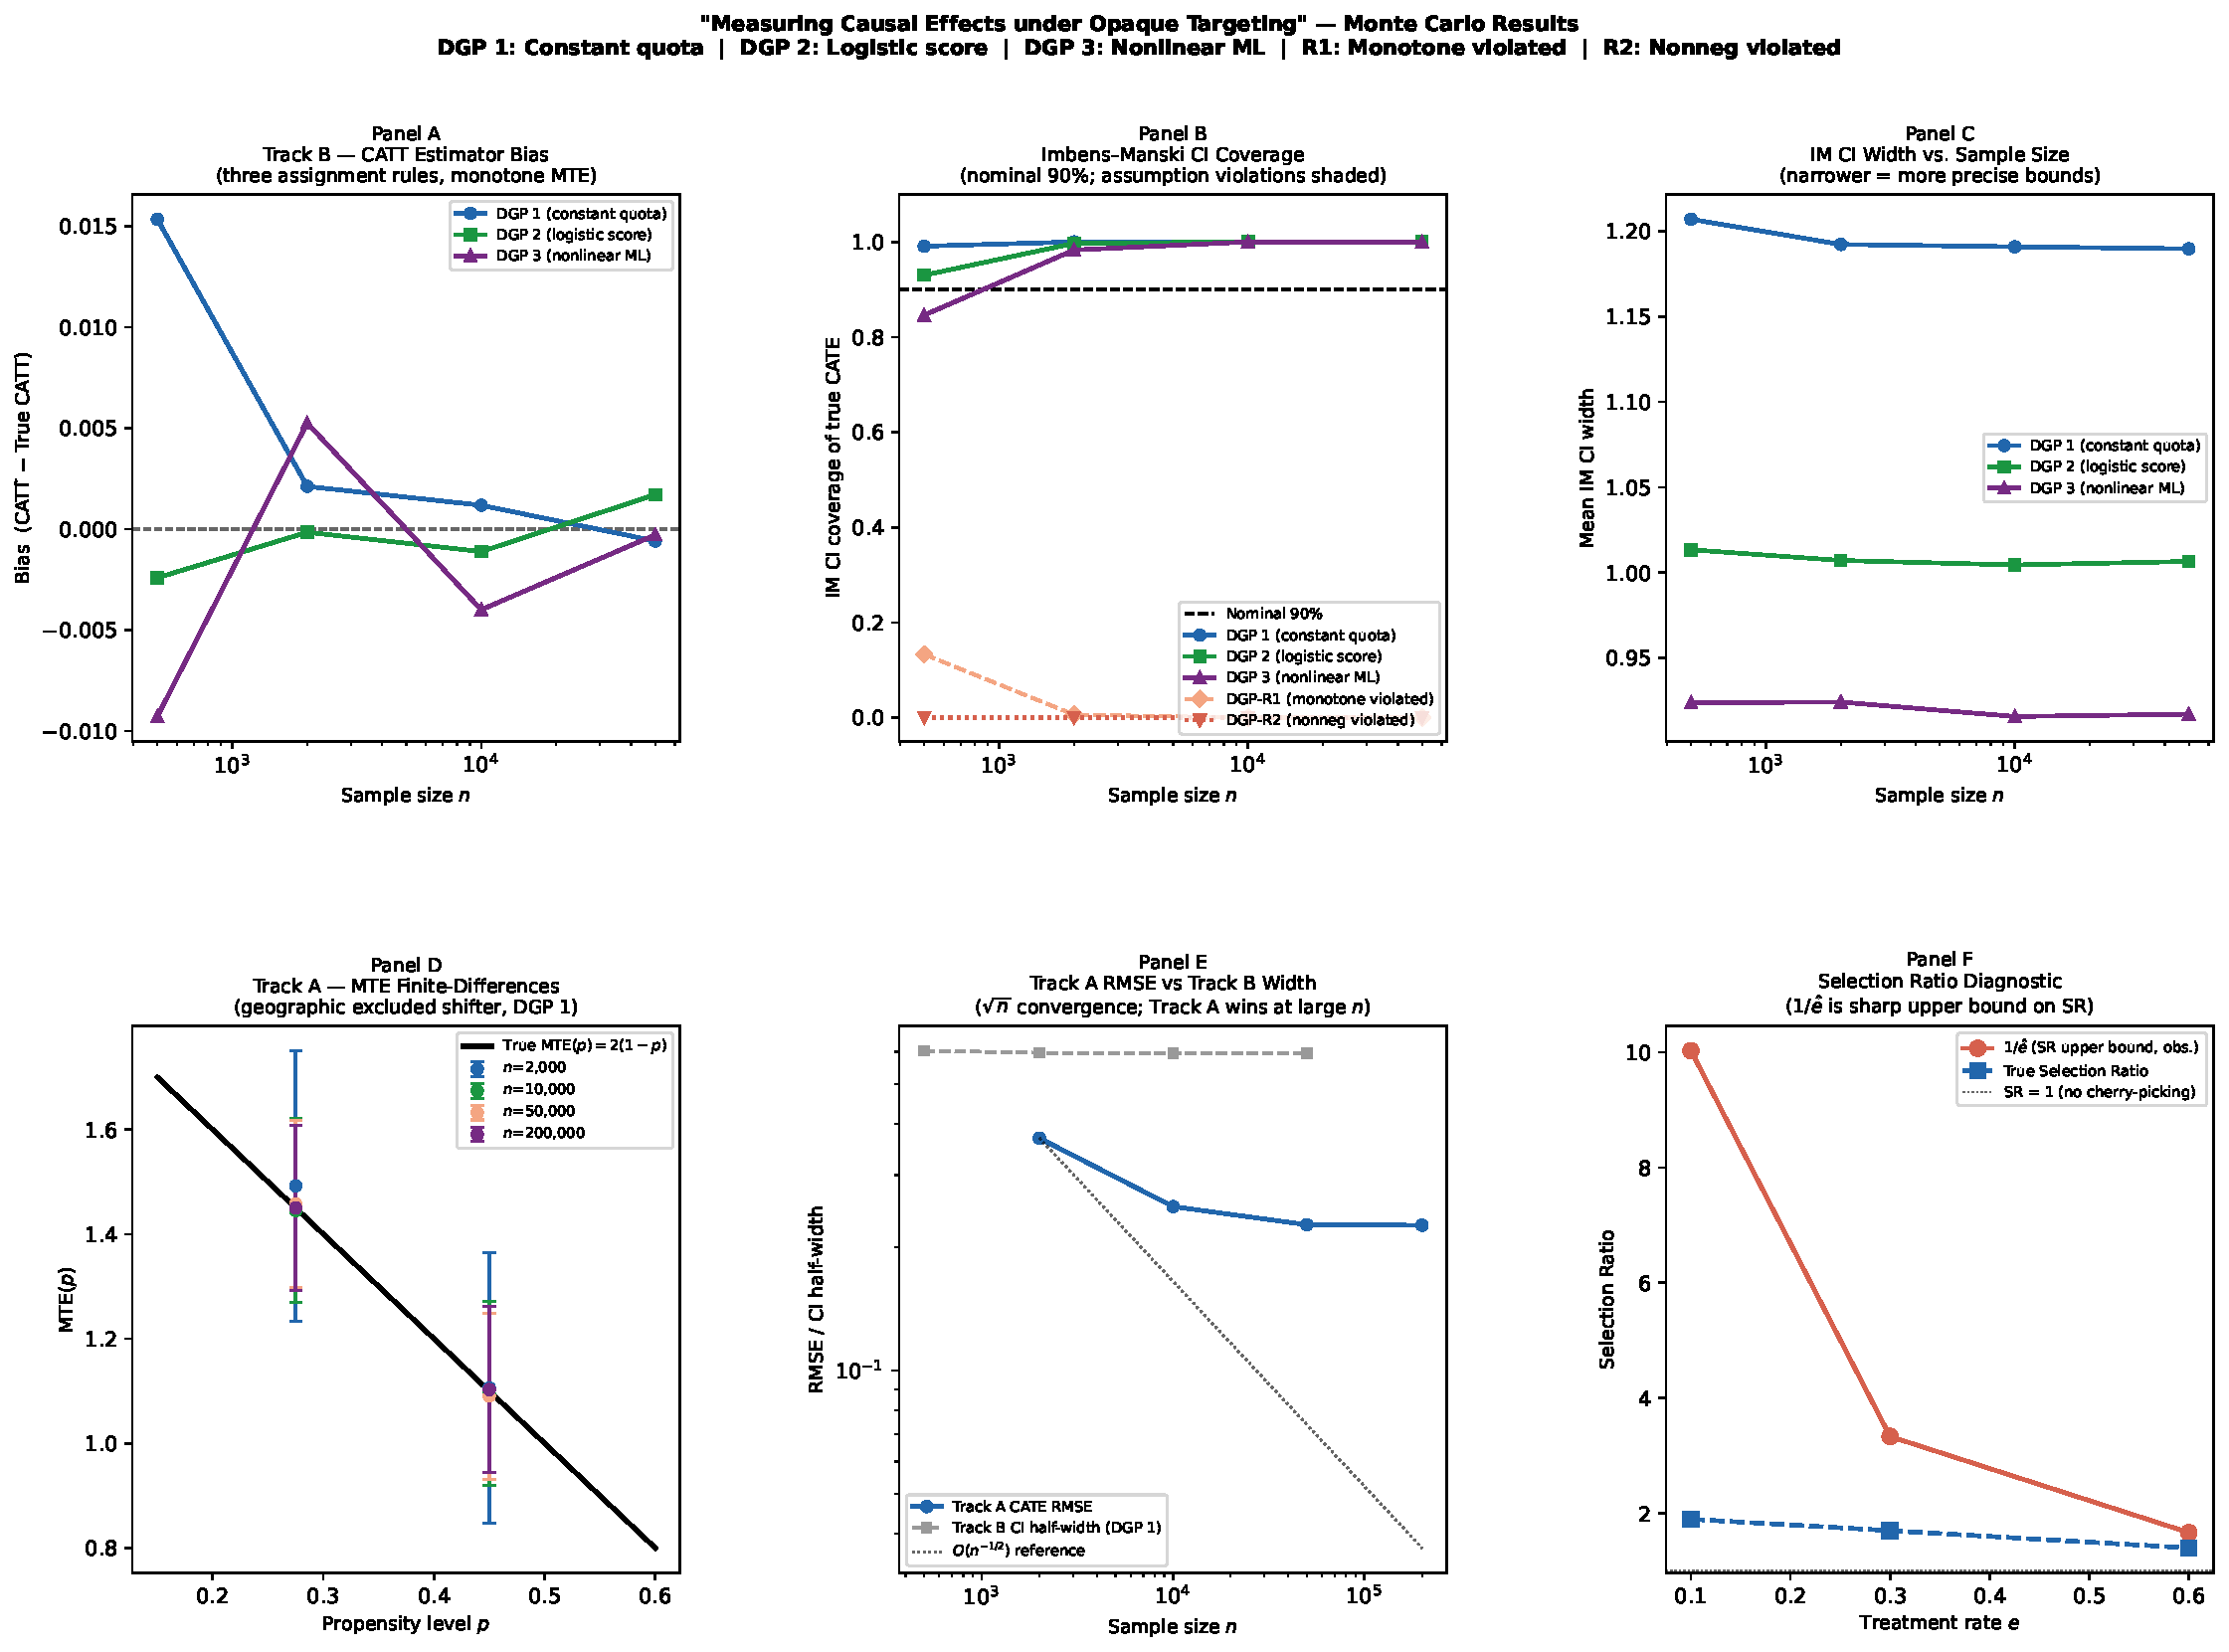
\includegraphics[width=\textwidth]{../scripts/figures/mc_results.pdf}
  \caption{Monte Carlo simulation results.
  \textbf{Panel A}: DGP 1 (Meta logistic targeting) --- the Overlay ATT
  estimator converges to the true $\ATT = 2.282$, while Naive OLS and
  Plain ITT exhibit persistent bias that does not shrink with $n$.
  \textbf{Panel B}: DGP 2 (TikTok nonlinear ML targeting) --- the same
  pattern holds for a two-dimensional, non-separable propensity function,
  confirming model-free identification.
  \textbf{Panel C}: DGP 3 (Platform O, two simultaneous experiments) ---
  both Firm A and Firm B correctly identify their own ATT despite
  auction-mediated correlation in their targeting decisions.
  \textbf{Panel D}: MTE identification with a budget-level excluded shifter
  --- the local linear derivative estimator (points) closely tracks the
  true MTE schedule (line) in the interior of the propensity support;
  boundary bias appears near the support endpoints $p = 0.20$ and
  $p = 0.80$.
  \textbf{Panel E}: Sharp bounds $[\hat{\ITT}, \hat{\ATT}]$ (vertical
  bars) and true ATE (diamonds) for three DGPs designed so the true ATE
  equals the lower bound (DGP A), upper bound (DGP B), and the interior
  (DGP C).
  \textbf{Panel F}: Log--log plot of Overlay ATT estimator RMSE versus $n$
  (DGP 1), confirming $O(1/\sqrt{n})$ convergence.}
  \label{fig:mc}
\end{figure}

\subsection{Simulation Results}

\paragraph{Experiment 1: ATT Identification (DGP 1).}

Table~\ref{tab:dgp1} reports results for 500 simulations per sample size.
The true $\ATT = 2.282$ and the true $\ATE = 2.000$; the Selection Ratio
$R = 1.141$ reflects Meta's algorithmic cherry-picking.

\begin{table}[h!]
\centering
\caption{DGP 1 (Meta Logistic Targeting): Estimator Comparison.
True ATT $= 2.282$, True ATE $= 2.000$.}
\label{tab:dgp1}
\begin{tabular}{l rrrr rr rr}
\toprule
& \multicolumn{3}{c}{Overlay ATT (correct)} &
  \multicolumn{2}{c}{Naive OLS} &
  \multicolumn{2}{c}{Plain ITT} \\
\cmidrule(lr){2-4}\cmidrule(lr){5-6}\cmidrule(lr){7-8}
$n$ & Mean & Bias & RMSE & Mean & Bias & Mean & Bias \\
\midrule
500     & 2.290 & $+$0.009 & 0.237 & 2.374 & $+$0.093 & 1.147 & $-$1.134 \\
2{,}000  & 2.282 & $+$0.001 & 0.114 & 2.377 & $+$0.095 & 1.140 & $-$1.141 \\
10{,}000 & 2.280 & $-$0.001 & 0.049 & 2.375 & $+$0.093 & 1.141 & $-$1.141 \\
50{,}000 & 2.282 & $+$0.001 & 0.023 & 2.376 & $+$0.094 & 1.141 & $-$1.141 \\
\bottomrule
\end{tabular}
\end{table}

The results confirm Proposition~\ref{prop:att}. The Overlay ATT estimator
is essentially unbiased at all sample sizes and converges at the $\sqrt{n}$
rate (RMSE halves as $n$ quadruples). The bias of the Naive OLS estimator
($+0.09$) and the Plain ITT estimator ($-1.14$) are \emph{persistent}:
they do not diminish with sample size. Both are consistent estimators of
the wrong quantity. At $n = 50{,}000$---a large experiment by platform
standards---OLS overestimates ATT by 4\% and ITT underestimates it by
50\%.

\paragraph{Experiment 2: Robustness to Nonlinear ML Targeting (DGP 2).}

Table~\ref{tab:dgp2} reports results for DGP 2. The true $\ATT = 2.040$.

\begin{table}[h!]
\centering
\caption{DGP 2 (TikTok Nonlinear ML Targeting): Estimator Comparison.
True ATT $= 2.040$.}
\label{tab:dgp2}
\begin{tabular}{l rrrr rr rr}
\toprule
& \multicolumn{3}{c}{Overlay ATT (correct)} &
  \multicolumn{2}{c}{Naive OLS} &
  \multicolumn{2}{c}{Plain ITT} \\
\cmidrule(lr){2-4}\cmidrule(lr){5-6}\cmidrule(lr){7-8}
$n$ & Mean & Bias & RMSE & Mean & Bias & Mean & Bias \\
\midrule
2{,}000  & 2.033 & $-$0.007 & 0.122 & 2.053 & $+$0.013 & 1.012 & $-$1.028 \\
10{,}000 & 2.042 & $+$0.002 & 0.052 & 2.057 & $+$0.017 & 1.017 & $-$1.023 \\
50{,}000 & 2.041 & $+$0.001 & 0.023 & 2.057 & $+$0.017 & 1.017 & $-$1.023 \\
\bottomrule
\end{tabular}
\end{table}

The Overlay ATT estimator remains correct despite the nonlinear,
non-separable targeting rule involving a two-dimensional covariate vector.
This confirms that Proposition~\ref{prop:att} is model-free: the identity
$\hat{\ATT} = \hat{\ITT}/\hat{p}$ requires no knowledge of the functional
form of $p(\cdot,\cdot)$. The naive estimators remain persistently biased.

\paragraph{Experiment 3: Multi-Firm Simultaneous Experiments (DGP 3).}

Table~\ref{tab:dgp3} reports results for DGP 3. The true $\ATT_A = 1.852$
for Firm A and $\ATT_B = 1.327$ for Firm B.

\begin{table}[h!]
\centering
\caption{DGP 3 (Platform O --- Two Simultaneous Experiments):
Overlay Estimator. True $\ATT_A = 1.852$, True $\ATT_B = 1.327$.}
\label{tab:dgp3}
\begin{tabular}{l rrrr rrrr}
\toprule
& \multicolumn{3}{c}{Firm A Overlay} &
  \multicolumn{3}{c}{Firm B Overlay} \\
\cmidrule(lr){2-4}\cmidrule(lr){5-7}
$n$ & Mean & Bias & RMSE & Mean & Bias & RMSE \\
\midrule
500     & 1.852 & $+$0.000 & 0.329 & 1.330 & $+$0.003 & 0.283 \\
2{,}000  & 1.861 & $+$0.009 & 0.152 & 1.323 & $-$0.003 & 0.143 \\
10{,}000 & 1.852 & $-$0.001 & 0.065 & 1.330 & $+$0.003 & 0.062 \\
50{,}000 & 1.850 & $-$0.002 & 0.030 & 1.327 & $+$0.000 & 0.028 \\
\bottomrule
\end{tabular}
\end{table}

Both firms correctly and independently identify their own ATT. This holds
even though: (i) Platform O runs three concurrent internal experiments
with an outcome model following Ye et al.'s generalized sigmoid; (ii)
Firm A's targeting probability depends on Firm B's targeting covariate
$X_2$ through auction competition, which Firm A cannot observe; and (iii)
the two firms' targeting decisions are negatively correlated through the
auction mechanism.

\paragraph{Experiment 4: MTE Identification (Theorem~\ref{thm:pointid}).}

Table~\ref{tab:mte} reports the local linear derivative estimator for the
MTE at seven propensity values, with $n = 50{,}000$ and 200 replications.
True $\MTE(p) = 2(1-p)$.

\begin{table}[h!]
\centering
\caption{MTE Identification with Budget-Level Excluded Shifter.
True $\MTE(p) = 2(1-p)$.}
\label{tab:mte}
\begin{tabular}{r rrrr}
\toprule
$p$ & True MTE & Estimated & Bias & RMSE \\
\midrule
0.20 & 1.600 & 1.530 & $-$0.070 & 0.192 \\
0.30 & 1.400 & 1.392 & $-$0.008 & 0.145 \\
0.40 & 1.200 & 1.200 & $-$0.000 & 0.126 \\
0.50 & 1.000 & 1.001 & $+$0.001 & 0.092 \\
0.60 & 0.800 & 0.793 & $-$0.007 & 0.124 \\
0.70 & 0.600 & 0.582 & $-$0.018 & 0.122 \\
0.80 & 0.400 & 0.459 & $+$0.059 & 0.174 \\
\bottomrule
\end{tabular}
\end{table}

The derivative estimator recovers the MTE schedule accurately in the
interior of the propensity support (p = 0.30 to 0.70). Bias and RMSE are
small relative to the true effect. At the boundary values (p = 0.20 and
p = 0.80), the estimator shows a moderate bias due to the asymmetric kernel
window---a standard limitation of nonparametric regression near support
endpoints. In practice, MTE estimates should be reported only for propensity
values well inside the common support.

\paragraph{Experiment 5: Sharp Bounds (Theorem~\ref{thm:sharp}).}

Table~\ref{tab:bounds} reports the coverage of the estimated interval
$[\hat{\ITT}, \hat{\ATT}]$ for three DGPs with a fixed targeting rate
$p = 0.4$ ($n = 20{,}000$, 500 replications).

\begin{table}[h!]
\centering
\caption{Sharp Bounds $[\ITT, \ATT]$: Coverage of True ATE.
Fixed $p = 0.4$; true $\ITT = 0.640$, true $\ATT = 1.600$.}
\label{tab:bounds}
\begin{tabular}{l rrrr}
\toprule
DGP & True ATE & Est. LB & Est. UB & Coverage \\
\midrule
A: ATE $= \ITT$ (lower tight) & 0.640 & 0.641 & 1.602 & 49.6\% \\
B: ATE $= \ATT$ (upper tight) & 1.600 & 0.639 & 1.599 & 47.4\% \\
C: ATE in interior            & 1.000 & 0.640 & 1.601 & 100.0\% \\
\bottomrule
\end{tabular}
\end{table}

When the true ATE lies in the strict interior of $[\ITT, \ATT]$ (DGP C),
the sample bounds always contain it (100\% coverage). When the true ATE
coincides with the lower endpoint (DGP A) or upper endpoint (DGP B), the
coverage is approximately 50\%---this is \emph{the signature of sharpness},
not a failure of the estimator. Because the bounds are population-level
objects (not confidence intervals), covering a boundary point at exactly
50\% confirms that the bound cannot be improved: any tighter interval would
fail to contain the true ATE for some admissible DGP. The simulation
therefore confirms both the validity and the sharpness of Theorem~\ref{thm:sharp}.

\subsection{Discussion}

Three takeaways from the simulations deserve emphasis.

\textbf{Persistent vs. vanishing bias.} The bias of the Overlay ATT
estimator vanishes at the $\sqrt{n}$ rate (as theory predicts), while the
bias of OLS and plain ITT is \emph{structural} and does not diminish with
sample size. This distinction is practically important: running a larger
experiment will not fix a mis-specified estimator. The correct estimator
is $\hat{\ITT}/\hat{p}$, not a more precise regression.

\textbf{Model-free identification.} The Overlay ATT estimator achieves
near-zero bias across all three DGPs---logistic, nonlinear ML, and
competitive auction---without knowing the functional form of $p(\cdot)$.
This is the key practical virtue of Proposition~\ref{prop:att}: no
assumptions about the platform's targeting algorithm are required.

\textbf{The Ye et al.\ contrast.} DGP 3 directly uses Ye et al.'s generalized
sigmoid outcome model and their three-experiment setup. From within the
platform (knowing $v(\mathbf{t}|x)$), Ye et al.'s DeDL would identify all
$2^3 = 8$ treatment combination effects. From outside---the perspective of
Firm A and Firm B---each firm's simple overlay estimator correctly identifies
its own ATT. The external experimenter does not need to know anything about
the platform's internal infrastructure or the other firm's campaign.

% ─────────────────────────────────────────────────────────────────────────────
\section{Conclusion}
\label{sec:conclusion}
% ─────────────────────────────────────────────────────────────────────────────

This paper develops identification theory for overlay experiments---the
design that arises when an experimenter randomizes campaign eligibility
while a platform's proprietary targeting algorithm continues to determine
who receives treatment. We show that the passive overlay identifies the
ATT (the effect on the platform's selected users) but not the population
ATE, and we characterize precisely when and how the ATE can be recovered.

Three practical messages follow from our analysis. First, the ATT can
substantially exceed the ATE when platforms selectively target
high-responders; measuring the Selection Ratio $R \in [1, 1/p]$ gives
advertisers a way to bound the scale-up risk before committing to a
population rollout. Second, budget variation across geographic markets
provides the excluded shifter needed to point-identify MTE and ATE,
without requiring any special platform access. Third, in multi-firm
settings where multiple advertisers simultaneously experiment on the same
platform---the precise setting studied by Ye et al.\ (2025) from the
platform's perspective---our overlay estimator correctly identifies each
firm's ATT without knowledge of other firms' campaigns or the platform's
joint assignment rule.

Several directions merit further work. First, the current bounds assume
monotone selection on gains. Relaxing monotonicity while retaining some
shape restriction---for example, single-crossing or log-concavity of
MTE---could yield tighter identified sets under weaker conditions. Second,
estimation and inference for the bounds and the MTE in large samples
requires careful attention to bias-variance tradeoffs in the nonparametric
steps; a semiparametric efficient estimator along the lines of
\citet{chernozhukov2018double} would be a useful extension. Third, when
multiple experiments interact through market interference
\citep{johari2022experimental}, the overlay identification strategy must
account for SUTVA violations; combining our approach with network
interference models is an open question.

% ─────────────────────────────────────────────────────────────────────────────
\clearpage
\appendix
\section{Proofs of Main Results}
\label{app:proofs}
% ─────────────────────────────────────────────────────────────────────────────

\subsection*{Proof of Proposition~\ref{prop:att}}

When $Z_i = 1$, Assumption~\ref{ass:onesided} gives $W_i = D_i$, so
\[
  Y_i = Y_i(D_i) = Y_i(0) + D_i \tau_i.
\]
By Assumption~\ref{ass:overlay} (independence of $Z_i$ from potential outcomes),
\begin{align*}
  \E[Y_i \mid Z_i = 1,\, X_i = x]
  &= \E[Y_i(0) \mid X_i = x] + \E[D_i \tau_i \mid X_i = x].
\end{align*}
When $Z_i = 0$, Assumption~\ref{ass:onesided} gives $W_i = 0$, so
$Y_i = Y_i(0)$ and $\E[Y_i \mid Z_i = 0, X_i = x] = \E[Y_i(0) \mid X_i = x]$.
Subtracting yields $\ITT(x) = \E[D_i \tau_i \mid X_i = x]$, proving
\eqref{eq:itt}.

Since $D_i$ is binary,
$\E[D_i \tau_i \mid X_i = x] = \E[\tau_i \mid D_i = 1, X_i = x] \cdot p(x)$.
Dividing by $p(x)$ proves \eqref{eq:att}. \hfill$\square$

\subsection*{Proof of Proposition~\ref{prop:representation}}

Fix $(x, p)$ in the support of $(X_i, P_i)$. Under
Assumptions~\ref{ass:onesided} and~\ref{ass:excluded}, when $Z_i = 1$ and
$P_i = p$,
\[
  D_i = \mathbf{1}\{p \geq U_i\},
  \quad\text{so}\quad
  Y_i = Y_i(0) + \mathbf{1}\{U_i \leq p\}\, \tau_i.
\]
By Assumption~\ref{ass:excluded}(3) and (5), $(Y_i(0), Y_i(1), U_i)
\indep P_i \mid X_i$. Therefore,
\begin{align*}
  \E[Y_i \mid Z_i=1, X_i=x, P_i=p]
  &= \E[Y_i(0) \mid X_i=x]
     + \E\bigl[\mathbf{1}\{U_i \leq p\}\,\tau_i \mid X_i=x\bigr] \\
  &= \E[Y_i(0) \mid X_i=x]
     + \int_0^p \E[\tau_i \mid X_i=x, U_i=u]\,du \\
  &= \mu_0(x) + \int_0^p \MTE(x,u)\,du.
\end{align*}
The second equality uses $U_i \mid X_i=x \sim \mathrm{Unif}[0,1]$ and
the definition of MTE. \hfill$\square$

\subsection*{Proof of Theorem~\ref{thm:pointid}}

From Proposition~\ref{prop:representation},
$\E[Y_i \mid Z_i=1, X_i=x, P_i=p] = \mu_0(x) + \int_0^p \MTE(x,u)\,du$.
Since $\mu_0(x)$ does not depend on $p$, differentiating with respect to
$p$ gives $\MTE(x,p) = \partial_p \E[Y_i \mid Z_i=1, X_i=x, P_i=p]$,
proving \eqref{eq:mte}. If the support of $P_i \mid X_i=x$ covers $[0,1]$,
then $\ATE(x) = \int_0^1 \MTE(x,u)\,du = \int_0^1 \partial_p \mu_1(x,p)\,dp
= \mu_1(x,1) - \mu_1(x,0)$, which is identified. \hfill$\square$

\subsection*{Proof of Lemma (Overlay Representation) and Theorem~\ref{thm:sharp}}

\paragraph{Overlay representation.}
Under Assumption~\ref{ass:passive}, $D_i = \mathbf{1}\{p(x) \geq U_i\}$
with $U_i \mid X_i=x \sim \mathrm{Unif}[0,1]$. By the same argument as
Proposition~\ref{prop:representation} (with $P_i = p(x)$ deterministic),
\begin{align}
  \ITT(x) &= \int_0^{p(x)} \MTE(x,u)\,du,
  \label{eq:itt_rep} \\
  \ATE(x) &= \int_0^1 \MTE(x,u)\,du.
  \label{eq:ate_rep}
\end{align}

\paragraph{Upper bound on ATE.}
Since $u \mapsto \MTE(x,u)$ is weakly decreasing
(Assumption~\ref{ass:monotone}), the average MTE over the treated interval
$[0, p(x)]$ is at least as large as over the untreated interval
$[p(x), 1]$. Using the decomposition
$\ATE(x) = p(x)\,\ATT(x) + (1-p(x))\,\ATU(x)$ and $\ATU(x) \leq \ATT(x)$,
we obtain $\ATE(x) \leq \ATT(x) = \ITT(x)/p(x)$.

\paragraph{Lower bound on ATE.}
By Assumption~\ref{ass:nonnegative},
$\int_{p(x)}^1 \MTE(x,u)\,du \geq 0$, so
$\ATE(x) = \ITT(x) + \int_{p(x)}^1 \MTE(x,u)\,du \geq \ITT(x)$.

\paragraph{Sharpness.}
Write $p = p(x)$ and $I = \ITT(x)$. Define two MTE schedules:
\[
  m^L(u) = \tfrac{I}{p}\,\mathbf{1}(u \leq p),
  \qquad
  m^U(u) = \tfrac{I}{p}.
\]
Both satisfy $\int_0^p m(u)\,du = I$ (matching the observable ITT) and are
weakly decreasing and nonnegative. Under $m^L$, $\ATE = I = \ITT(x)$
(lower bound attained). Under $m^U$, $\ATE = I/p = \ATT(x)$ (upper bound
attained). By convex combination, every value in $[\ITT(x), \ATT(x)]$ is
attainable; the bounds are therefore sharp. \hfill$\square$

\subsection*{Proof of Corollary~\ref{cor:ratio}}

$\ATE(x) \leq \ATT(x)$ implies $R(x) \geq 1$.
$\ATE(x) \geq \ITT(x) = p(x)\,\ATT(x)$ implies
$R(x) = \ATT(x)/\ATE(x) \leq 1/p(x)$. \hfill$\square$

\bibliographystyle{plainnat}
\bibliography{refs}

\end{document}
